\section{Composition of Linear Transformations and Matrix Multiplication}
\begin{enumerate}
\item \begin{enumerate}
\item It should be $[UT]_{\alpha }^{\gamma }=[T]_{\alpha }^{\beta }[U]_{\beta }^{\gamma }$.
\item Yes. That's Theorem 2.14.
\item No. In general $\beta $ is not a basis for $V$.
\item Yes. That's Theorem 2.12.
\item No. It will be true when $\beta =\alpha $.
\item No. We have $\left(\begin{array}{cc}0&1\\1&0\end{array}\right) ^2=I$.
\item No. $T$ is a transformation from $V$ to $W$ but $L_A$ can only be a transformation from $\mathbb{F}^m$ to $\mathbb{F}^n$.
\item No. We have $\left(\begin{array}{cc}0&1\\0&0\end{array}\right) ^2=I$.
\item Yes. That's Theorem 2.15.
\item Yes. Since $\delta_{ij}=1$ only when $i=j$, we have $A_{ij}=\delta_ij$.
\end{enumerate}
\item \begin{enumerate}
\item \[A(2B+3C)=\left(\begin{array}{ccc}20&-9&18\\5&10&8\end{array}\right).\]
\[(AB)D=A(BD)=\left(\begin{array}{c}29\\-26\end{array}\right).\]
\item \[A^t=\left(\begin{array}{ccc}2&-3&4\\5&1&2\end{array}\right).\]
\[A^tB=\left(\begin{array}{ccc}23&19&0\\26&-1&10\end{array}\right).\]
\[BC^t=\left(\begin{array}{c}12\\16\\29\end{array}\right).\]
\[CB=\left(\begin{array}{ccc}27&7&9\end{array}\right).\]
\[CA=\left(\begin{array}{ccc}20&26\end{array}\right).\]
\end{enumerate}
\item \begin{enumerate}
\item We can calculate that $[U]_{\beta}^{\gamma}=\left(\begin{array}{ccc}1&1&0\\0&0&1\\1&-1&0\end{array}\right)$ and $[T]_{\beta}=\left(\begin{array}{ccc}2&3&0\\0&3&6\\0&0&4\end{array}\right)$ and finally \[[UT]_{\beta}^{\gamma}=\left(\begin{array}{ccc}2&6&6\\0&0&4\\2&0&-6\end{array}\right).\]
\item We can calculate $[h(x)]_{\beta}=\left(\begin{array}{c}3\\-2\\1\end{array}\right)$ and \[[U(h(x))]_{\beta}=[U]_{\beta}^{\gamma}[h(x)]_{\beta}\left(\begin{array}{c}1\\1\\5\end{array}\right).\]
\end{enumerate}
\item \begin{enumerate}
\item $[T(A)]_{\alpha}=\left(\begin{array}{c}1\\-1\\4\\6\end{array}\right).$
\item $[T(f(x))]_{\alpha}=\left(\begin{array}{c}-6\\2\\0\\6\end{array}\right).$
\item $[T(A)]_{\gamma}=\left(\begin{array}{c}5\end{array}\right).$
\item $[T(f(x))]_{\gamma}=\left(\begin{array}{c}12\end{array}\right).$
\end{enumerate}
\item \begin{description}
\item[(b)] We have 
\begin{align*}
(a(AB))_{ij}&=a\sum_{k=1}^n{A_{ik}B_{kj}}\\
&\sum_{k=1}^n{aA_{ik}B_{kj}}=((aA)B)_{ij}\\
&\sum_{k=1}^n{A_{ik}aB_{kj}}=(A(aB))_{ij}
\end{align*}
\item[(d)] We have $[I(v_i)]_{\alpha}=e_i$ where $v_i$ is the $i$-th vector of $\beta $.
\item[Corollary.] We have by Theorem 2.12
\[A(\sum_{i=1}^k{a_iB_i})=\sum_{i=1}^k{A(a_iB_i)}=\sum_{i=1}^k{a_iAB_i}\]
and
\[(\sum_{i=1}^k{a_iC_i})A=\sum_{i=1}^k{(a_iC_i)A}=\sum_{i=1}^k{a_iC_iA}.\]
\end{description}
\item We have $(Be_j)_i=\sum_{k=1}^n{B_{ik}(e_j)_i}=B_{ij}$, since $(e_j)_i=1$ only when $i=j$ and it's $0$ otherwise.
\item \begin{description}
\item[(c)] Just check that for all vector $v\in \mathbb{F}^n$ we have $L_{A+B}(v)=(A+B)v=Av+Bv=L_A(v)+L_B(v)$ and $L_{aA}(v)=aA(v)=aL_A(v)$.
\item[(f)] For all vector $v\in \mathbb{F}^n$ we have $L_{I_n}(v)=I_n(v)=v$.
\end{description}
\item In general we may set $T_1,T_2\in \mathcal{L}(X,Y)$ and $U_1,U_2\in \mathcal{L}(W,X)$, and $S\in \mathcal(V,W)$, and thus we have the following statements.
\begin{enumerate}
\item $T_1(U_1+U_2)=TU_1+TU_2$ and $(U_1+U_2)T=U_1T+U_2T$.
\item $T_1(U_1S)=(T_1U_1)S$.
\item $TI_X=I_YT=T$.
\item $a(T_1U_1)=(aT_1)U_1=T_1(aU_1)$ for all scalars $a$.
\end{enumerate}
To prove this, just map arbitrary vector in domain by linear transformations and check whether the vectors producted by different transformations meet.
\item Take $A=\left(\begin{array}{cc}0&1\\0&1\end{array}\right)$ and $B=\left(\begin{array}{cc}1&1\\0&0\end{array}\right)$ and $U=L_A$ and $T=L_B$.
\item If $A$ is a diagonal matrix then $A_{ij}\neq 0$ only when $i=j$. Hence we have $A_{ij}=\delta_{ij}A_{ij}$. Conversely, if $A$ is not diagonal, we can find $A_{ij}\neq 0$ for some $i,j$ and $i\neq j$. Thus we have $\delta_{ij}A_{ij}=0\neq A_{ij}$.
\item If $T^2=T$ we may pick $y\in R(T)$ and thus we have $y=T(x)$ for some $x$ and $T(y)=T(T(x))=T^2(x)=0$. Hence we conclude that $y\in N(T)$. Conversely if we have $R(T)\subset N(T)$, we have $T^2(x)=T(T(x))=0$ since $T(x)$ is an element in $R(T)$ and hence in $N(T)$.
\item \begin{enumerate}
\item If $UT$ is injective, we have that $UT(x)=0$ implies $x=0$. Thus we have that if $T(x)=0$ we also have $UT(x)=0$ and hence $x=0$. So $T$ is injective. But $U$ may not be injective. For example, pick $U(x,y,z)=(x,y)$, a mapping from $\mathbb{R}^3$ to $\mathbb{R}^2$, and $T(x,y)=(x,y,0)$, a mapping from $\mathbb{R}^2$ to $\mathbb{R}^3$.
\item If $UT$ is surjective, we have that for all $z\in Z$ there is a vector $x\in V$ such that $UT(x)=z$. Thus we have that if for all $z\in Z$ we have $z=U(T(x))$ and hence $U$ is surjective. But $T$ may not surjective. The example in the previous question could also be the example here.
\item For all $z\in Z$, we can find $z=U(y)$ for some $y\in W$ since $U$ is surjective and then find $y=T(x)$ for some $x\in V$ since $T$ is surjective. Thus we have $z=UT(x)$ for some $x$ and hence $UT$ is surjective. On the other hand, if $UT(x)=0$, this means $T(x)=0$ since $U$ is injective and $x=0$ since $T$ is injective.
\end{enumerate}
\item It's natural that we have tr$(A)=$tr$(A^t)$ since $A_{ii}=A^t_{ii}$ for all $i$. On the other hand we have 
\begin{align*}
\mathrm{tr}(AB)&=\sum_{i=1}^n{(AB)_{ii}}=\sum_{i=1}^n{\sum_{k=1}^n{A_{ik}B_{ki}}}\\
&=\sum_{k=1}^n{\sum_{ik=1}^n{B_{ki}A_{ik}}}=\sum_{k=1}^n{(BA)_{kk}}\\
&=\mathrm{tr}(BA).
\end{align*}
\item \begin{enumerate}
\item We can write 
\[Bz=\left(\begin{array}{c}\sum_{j=1}^p{a_jB_{1j}}\\\sum_{j=2}^p{a_jB_{2j}}\\ \vdots \\\sum_{j=1}^p{a_jB_{nj}}\end{array}\right)\]
\[=\sum_{j=1}^p{a_j\left(\begin{array}{c}B_{1j}\\B_{2j}\\ \vdots \\B_{nj}\end{array}\right)}=\sum_{j=1}^p{a_jv_j}.\]
\item This is the result of Theorem 2.13(b) and the previous exercise.
\item This is instant result of the fact that $wA=A^tw^t$.
\item This is also because $AB=B^tA^t$.
\end{enumerate}
\item Let $v_t$ be the $t$-th column vector of A and we have $v_j=\sum_{t\neq j}{a_tv_t}$. Thus we have $Mv_j=\sum_{t\neq j}{a_tMv_t}$. And hence we get the desired result since $Mv_t$ is the column vector of $MA$.
\item \begin{enumerate}
\item Since we know $R(T)$ is a $T$-invariant space, we can view $T$ as a mapping from $R(T)$ to $R(T)$ and call this restricted mapping $T|_{R(T)}$. So now we have that 
\[\mathrm{dim}R(T)=\mathrm{rank}(T)=\mathrm{rank}(T^2)=\mathrm{dim}(T(T(V))\]
\[=\mathrm{dim}(T(R(T))=\mathrm{rank}(T|_{R(T)}).\]
 And so the mapping $T|_{R(T)}$ is surjective and hence injective with the help of the fact $R(T)$ is finite dimensional. This also means $N(T|_{R(T)}=R(T)\cap N(T)={0}$. This complete the proof of the first statement. For the other, it's sufficient to say that $R(T)+N(T)=V$. But this is instant conclusion of the fact that $R(T)+N(T)\subset V$ and that 
\[\mathrm{dim}(R(T)+N(T))=\mathrm{dim}(R(T))+\mathrm{dim}(N(T))-\mathrm{dim}(R(T)\cap N(T))\]
\[=\mathrm{dim}(R(T))+\mathrm{dim}(N(T))=\mathrm{dim}(V).\]
\item In general we have rank$(T^{s+1})\leq $rank$(T^s)$ since the fact $T^{s+1}(V)=T^s(R(T))\subset T^s(V)$. But the integer rank$(T^s)$ can only range from $0$ to dim$(V)$. So there must be some integer $k$ such that 
\[\mathrm{rank}(T^k)=\mathrm{rank}(T^{k+1}).\]
 And this means $T^{k+1}(V)=T^k(V)$ and hence $T^s(V)=T^k(V)$ for all $s\geq k$. Since $2k\geq k$, we can conclude that rank$(T^k)=$rank$(T^{2k})$ and hence we have $V=R(T^k)\oplus N(T^k)$ by the previous exercise.
\end{enumerate}
\item If $T=T^2$, then we have $V=\{y:T(y)=y\}+N(T)$ since $x=T(x)+(x-T(x))$ and we have $T(T(x))=T(x)$ and $T(x-T(x))=T(x)-T(x)=0$. On the other hand, we have if $x\in \{y:T(y)=y\}\cap N(T)$ then we also have $x=T(x)=0$. So by arguments above we have $V=\{y:T(y)=y\}\oplus N(T)$. Finally we have that $T$ must be the projection on $W_1$ along $W_2$ for some $W_1$ and $W_2$ such that $W_1\oplus W_2=V$.
\item Let $A$, $B$, and $C$ be $m\times n$, $n\times p$, and $p\times q$ matrices respectly. Next we want to claim that $(AB)C=A(BC)$ since 
\begin{align*}
((AB)C)_{ij}&=\sum_{k=1}^p{(AB)_{ik}C_{kj}}=\sum_{k=1}^p{(\sum_{l=1}^n{A_{il}B_{lk}})C_{kj}}\\
&=\sum_{k=1}^p{\sum_{l=1}^n{A_{il}B_{lk}C_{kj}}}=\sum_{l=1}^n{\sum_{k=1}^p{A_{il}B_{lk}C_{kj}}}\\
&=\sum_{l=1}^n{A_{il}(\sum_{k=1}^p{B_{lk}C_{kj}})}=\sum_{l=1}^n{A_{il}(BC)_{lj}}=(A(BC))_{ij}.
\end{align*}

For the following questions, I would like to prove them in the languague of Graph Theory. So there are some definitions and details in Appendices.
\item Let $G=\mathcal{G}(B)$ be the graph associated to the symmetric matric $B$. And $(B^3)_{ii}$ is the number of walk of length $3$ from $i$ to $i$. If $i$ is in some clique, then there must be a walk of length $3$ from $i$ back to $i$ since a clique must have number of vertex greater than $3$. Conversely, if $(B^3)_{ii}$ is greater than zero, this means there is at least one walke of length $3$ from $i$ to $i$, say $i\rightarrow j\rightarrow k\rightarrow i$. Note that $i$, $j$, and $k$ should be different vertices since length is $3$ and there is no loop. So $i$, $j$, and $k$ must be a triangle, this means three vertices adjacent to each others. So $i$ is contained in $\{i,j,k\}$ and so contained in some clique.
\item We can draw the associated digraph and find the cliques as follow:
\begin{center}
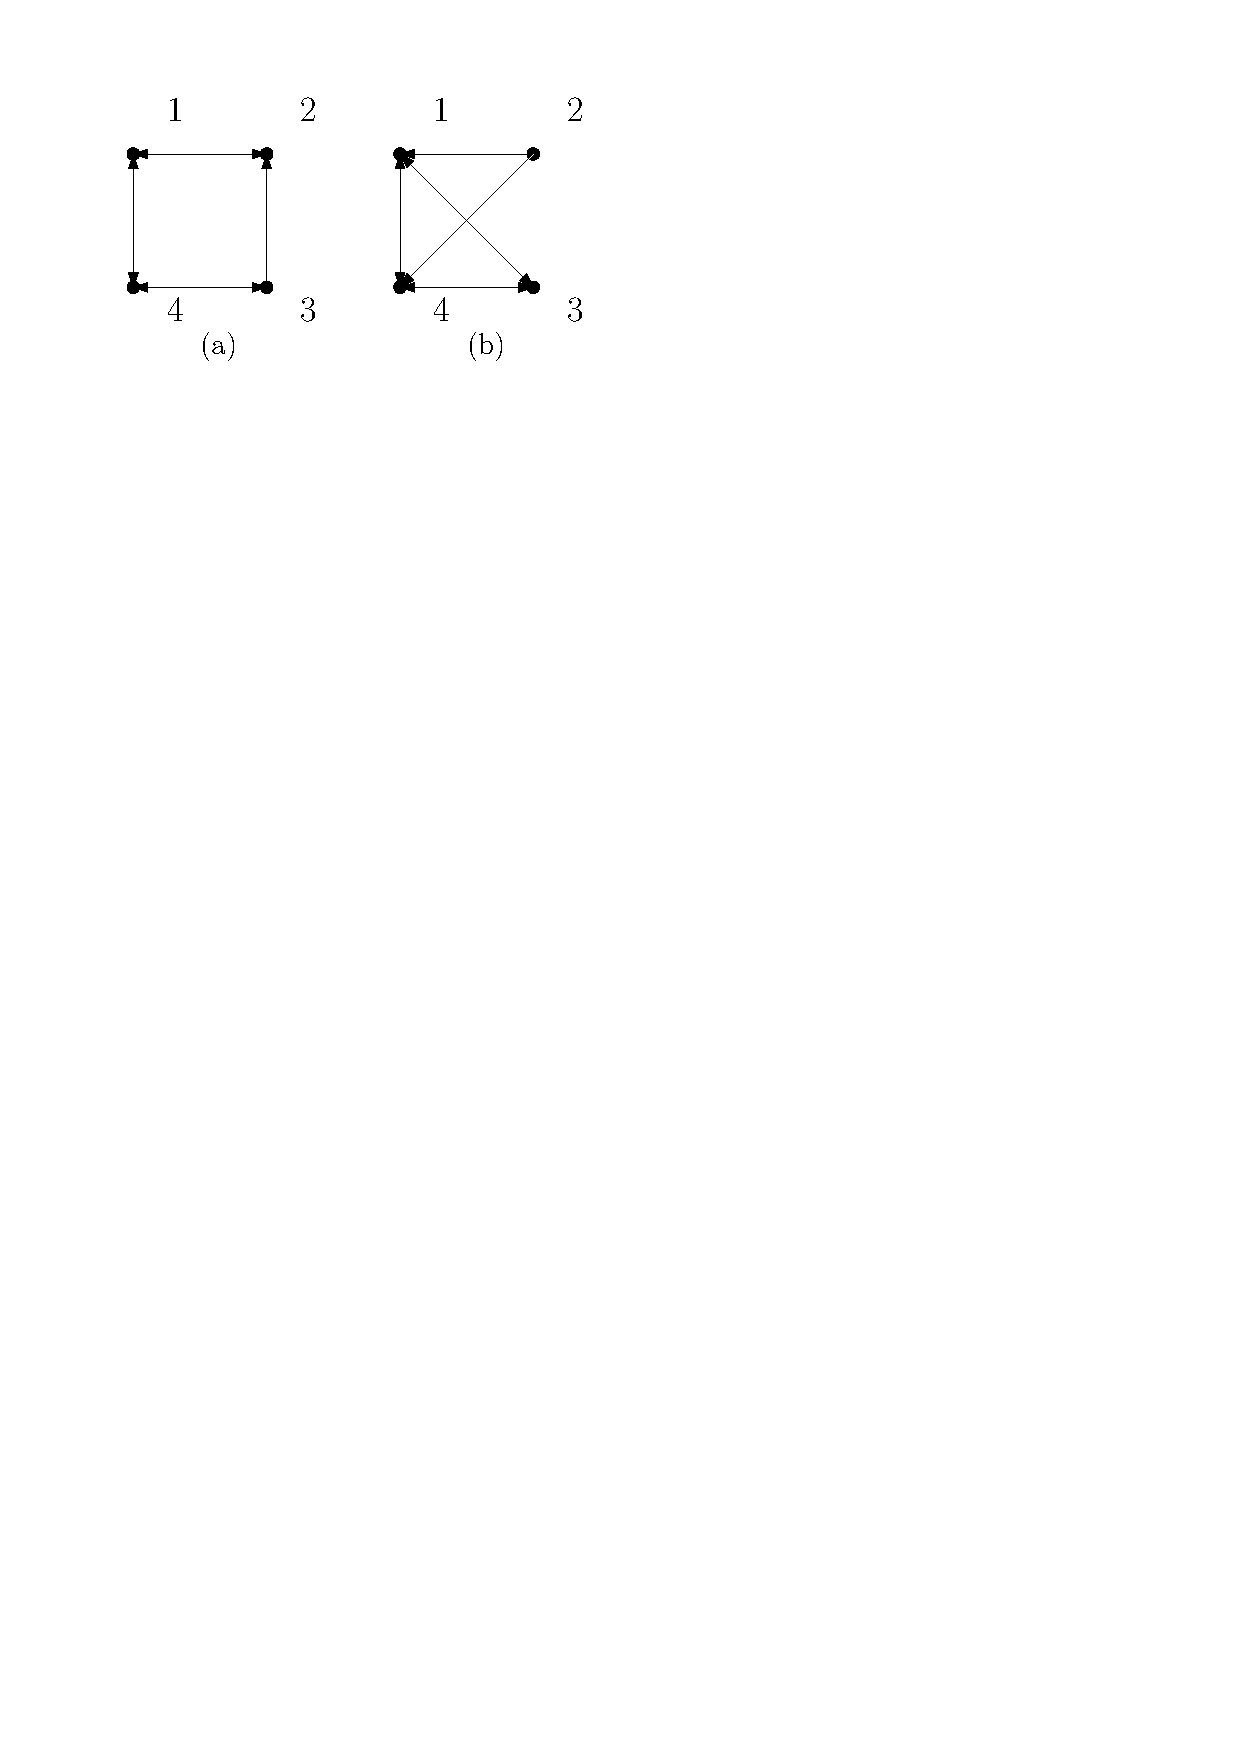
\includegraphics[scale=0.7]{2-4-20}
\end{center}
\begin{enumerate}
\item There is no clique.
\item The only clique would be the set $\{1,3,4\}$.
\end{enumerate}
\item A vertex $v$ in a tournament is called a \textbf{king} if $v$ can reach all other vertices within two steps. That is, for all vertex $u$ other than $v$, we have either $v\rightarrow u$ or $v\rightarrow w \rightarrow u$ for some $w$. So $(A+A^2)_{ij}>0$ is equivalent to that $i$ can reach $j$ within two steps. And the statement of this question also means that every tournament exists a king.

To prove this statement, we can begin by arbitrary vertex $v_1$. If $v_1$ is a king, then we've done. If $v_1$ is not a king, this means $v_1$ can not reach some vertex, say $v_2$, within two steps. Now we have that $d^+(v_2)>d^+(v_1)$ since we have $v_2\rightarrow v_1$ and that if $v_1\rightarrow w$ for some $w$ then we have $v_2\rightarrow w$ otherwise we'll have that $v_1\rightarrow w \rightarrow v_2$. Continuing this process and we can find $d^+(v_1)<d^+(v_2)<\cdots $ and terminate at some vertex $v_k$ since there are only finite vertces. And so $v_k$ would be a king.
\item We have $G=\mathcal{G}(A)$ is a tournament drawn below. And every vertex in this tournament could be a king.
\begin{center}
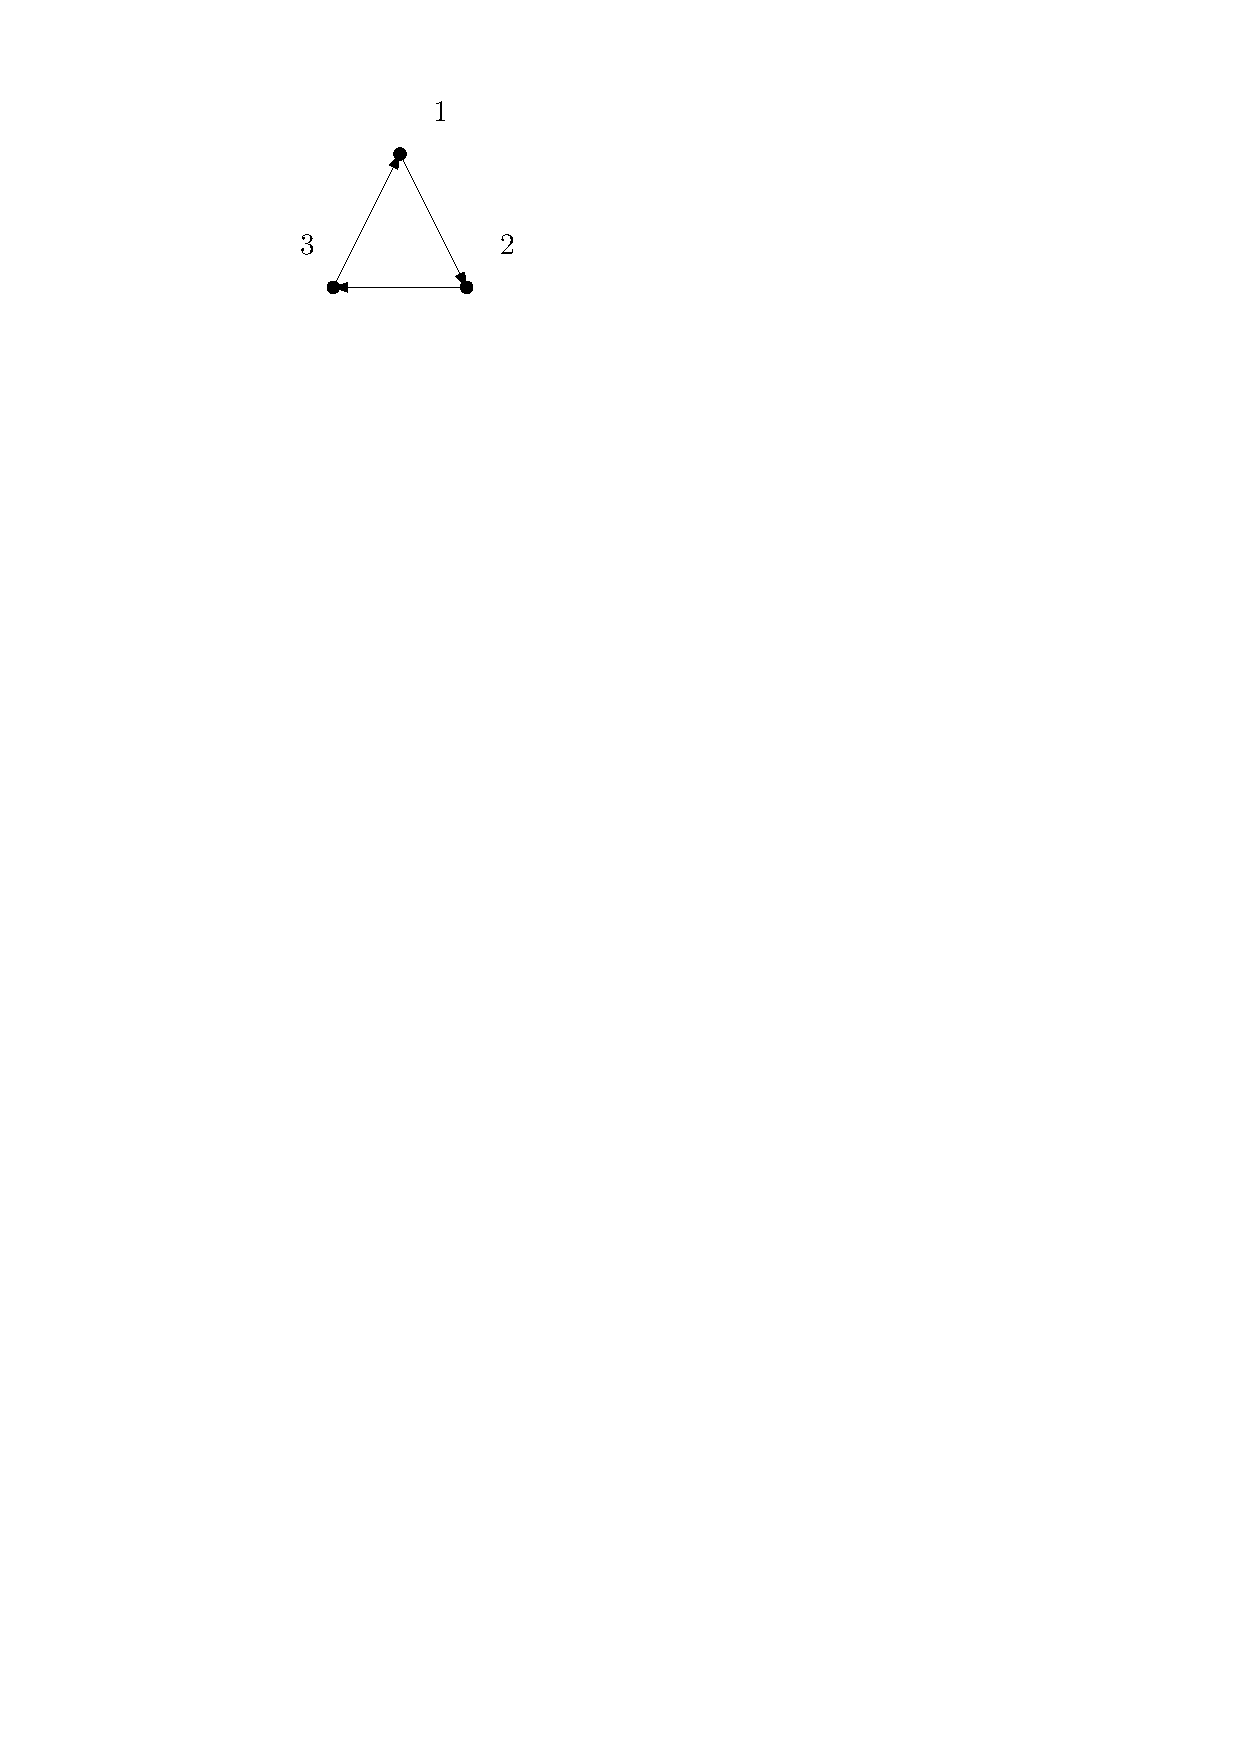
\includegraphics[scale=0.7]{2-4-22}
\end{center}
\item The number of nonzero entries would be the number of the edges in a tournament. So it would be $n(n-1)/2$.
\end{enumerate}